\documentclass{article}
\usepackage{float}
\usepackage{circuitikz}
\usepackage{cite}
\usepackage{amsmath,amssymb,amsfonts,amsthm}
\usepackage{algorithmic}
\usepackage{graphicx}
\usepackage{textcomp}
\usepackage{xcolor}
\usepackage{txfonts}
\usepackage{listings}
\usepackage{amsmath}
\usepackage{enumitem}
\usepackage{mathtools}
\usepackage{gensymb}
\usepackage{comment}
\usepackage[breaklinks=true]{hyperref}
\usepackage{tkz-euclide} 
\usepackage{listings}
\usepackage{gvv}        

%Enumering lower case roman numerals
%\renewcommand{\theenumi}{\roman{enumi}}   
%\renewcommand{\labelenumi}{\theenumi)}


\begin{document}

\title{ FILTER DESIGN ASSIGNMENT}
\author{EE23BTECH11011- Batchu Ishitha$^{*}$% <-this % stops a space
}
\maketitle

\bigskip

\renewcommand{\thefigure}{\theenumi}
\renewcommand{\thetable}{\theenumi}
%\renewcommand{\theequation}{\theenumi}

\section{\textbf{INTRODUCTION}}
We are supposed to design the equivalent FIR and IIR filter realizations for  given filter number.  
This is a bandpass filter whose specifications are available below.

\section{\textbf{Filter Specifications}}
The sampling rate for the filter has been specified as $F_s =  48$ kHz.	If the un-normalized  discrete-time (natural) frequency is F, the corresponding normalized digital filter (angular) frequency is given by $\omega = 2\pi\left(\frac{F}{F_s}\right)$.

\subsection{\textbf{The Digital Filter}}

\begin{enumerate}

\item {\em Passband:}  The passband of filter number $j$, is from \{4 + 0.6(j)\}kHz
to \{4 + 0.6(j+2)\}kHz where 
\begin{align}
    j=\brak{r-11000} \mod \sigma
\end{align}
where $\sigma$ is sum of digits of roll number and $r$ is roll number.\\
\begin{align}
    r&=11011\\
    \sigma  &= 4\\
    j&=3
\end{align}  
Substituting $j = 3$ gives the passband range for our bandpass filter as $5.8$ kHz - $7$ kHz. 
 Hence, the un-normalized discrete time filter passband frequencies are $F_{p1} = 7$ kHz
and $F_{p2} = 5.8$ kHz.  The corresponding normalized digital filter passband frequencies are

\begin{align}
\omega_{p1} = 2\pi\frac{F_{p1}}{F_s}  = 0.29\pi  \\
 \omega_{p2} = 2\pi\frac{F_{p2}}{F_s}  = 0.24 \pi
\end{align}  
 The centre frequency is then given by  
 \begin{align}
 \omega_c = \frac{\omega_{p1} + \omega_{p2}}{2} = 0.265\pi.  
 \end{align}

\item {\em Tolerances:}  The passband ($\delta_1$) and stopband ($\delta_2$) tolerances are given to
be equal, so we let $\delta_1 = \delta_2 = \delta = 0.15$.

\item {\em Stopband:}  The {\em transition band} for bandpass filters is $\Delta F = 0.3$ kHz on either side of the passband.
Hence, the un-normalized {\em stopband} frequencies are  
\begin{align}
F_{s1} = 7 + 0.3 = 7.3 kHz \\
F_{s2} = 5.8- 0.3 = 5.5 kHz.
 \end{align} 
The corresponding normalized frequencies are
\begin{align}
\omega_{s1} = 0.3041 \pi \\
\omega_{s2} =  0.2292\pi.
\end{align}
\end{enumerate}

\subsection{\textbf{The Analog filter}} \label{2.2}
In the bilinear transform, the analog filter frequency ($\Omega$) is related to the corresponding digital filter frequency ($\omega$) as
\begin{align}
\Omega = \tan \frac{\omega}{2}.
\end{align} 
 Using this relation, we obtain the analog passband and stopband frequencies as $\Omega_{p1} = 0.4899$, $\Omega_{p2} = 0.3959$ and $\Omega_{s1} = 0.5177$, $\Omega_{s2} = 0.3764$
respectively.

\section{\textbf{The IIR Filter Design}}
{\em Filter Type:}  We are supposed to design filters whose stopband is monotonic and passband equiripple.  
Hence, we use the {\em Chebyschev approximation} to design our bandpass IIR filter.

\subsection{\textbf{The Analog filter}} 
\begin{enumerate}

\item {\em Low Pass Filter Specifications:}  If $H_{a, BP}(j\Omega)$ be the desired analog band
pass filter,  with the specifications provided in Section \ref{2.2} , and $H_{a,LP}(j\Omega_L)$ 
be the equivalent low pass filter, then
\begin{equation}
\label{transition}
\Omega_L = \frac{\Omega^2 - \Omega_0^2}{B\Omega}
\end{equation}

%\begin{equation}
%H_{a, BP}(j\Omega) =  H_{a,LP}(j\Omega_L) \vert_{ \Omega_L = 
%\frac{\Omega^2 - \Omega_0^2}{B\Omega}},
%\end{equation}
where $\Omega_0 = \sqrt{\Omega_{p1}\Omega_{p2}} = 0.4404$ and $B = \Omega_{p1} - \Omega_{p2} = 0.094$. \\
 The low pass filter has the passband edge at $\Omega_{Lp} = 1$ and stopband edges at 
 \begin{align}
 \Omega_{Ls_1} = 1.5219 \\
 \Omega_{Ls_2} = -1.4775
 \end{align} 
 We choose the stopband edge of the analog low pass filter as 
 \begin{align}
 \Omega_{Ls} = \mbox{min}(\vert \Omega_{Ls_1}\vert,\vert \Omega_{Ls_2}\vert) = 1.4775.
 \end{align}

\item {\em The Low Pass Chebyschev Filter Paramters:}  The magnitude squared of the Chebyschev low pass filter is given by 
\begin{equation}
\label{lpfirst}
\vert H_{a,LP}(j\Omega_L)\vert^2 = \frac{1}{1 + \epsilon^2c_N^2(\Omega_L/\Omega_{Lp})}
\end{equation}
Since $\Omega_{Lp} = 1$, (\ref{lpfirst}) may be rewritten as
\begin{equation}
\label{lpsecond}
\vert H_{a,LP}(j\Omega_L)\vert^2 = \frac{1}{1 + \epsilon^2c_N^2(\Omega_L)}
\end{equation}
where 
\begin{align}
c_N(x) &= \cosh(N \cosh^{-1}x) \\
c_0(x) &=  1 \\
c_1(x) &=  x
\end{align}
and the integer $N$, which is the order of the filter, and $\epsilon$ are design paramters. 
 There exists a recurssive relation from which all the polynomials can be found out.
\begin{align}
    c_{N+2} &= 2xc_{N+1} - c_{N}  \label{eq:cheby_poly_relation}
\end{align}
Imposing the band restrictions on \eqref{lpfirst} \\
\begin{align}
    \vert H_{a,LP}(j\Omega_L)\vert^2 < \delta_{2} \hspace{5pt} \text{for}\hspace{5pt} \Omega_L = \Omega_{Ls}\\
    1-\delta_{1}<\vert H_{a,LP}(j\Omega_L)\vert^2 < 1 \hspace{5pt} \text{for}\hspace{5pt} \Omega_L = \Omega_{Lp}
\end{align}
we obtain :
\begin{eqnarray}
\label{lpdesign}
\frac{\sqrt{D_2}}{c_N(\Omega_{Ls})} \leq \epsilon \leq \sqrt{D_1}, \nonumber \\
N \geq \left\lceil \frac{\cosh^{-1}\sqrt{D_2/D_1}}{\cosh^{-1}\Omega_{Ls}} \right\rceil,
\end{eqnarray}
where $D_1 = \frac{1}{(1 - \delta)^2}-1$ and $D_2 = \frac{1}{\delta^2} - 1$ and $\left \lceil . \right \rceil$ is known as the ceiling operator.\\ 
\begin{table}[H]
    \centering
    \renewcommand\thetable{1}
    \setlength{\extrarowheight}{9pt}
    \resizebox{0.51\textwidth}{!}{
    \begin{tabular}{|c|c|c|}
    \hline
    \textbf{$r\brak{i}$} & \textbf{$p\brak{i}$} & \textbf{$k\brak{i}$} \\ \hline
    $0.58129538 -2.51766121j$ &0.13676769 +0.19533079j&$2.02482078$  \\ \hline
    $0.58129538 +2.51766121j$ &0.13676769 -0.19533079j&$-$  \\ \hline
    $-0.40482158+0.3262658j$ &0.188968140+0.6515556j&$-$  \\ \hline
    $-0.40462158-0.3262658j$ &0.188968140-0.6515556j&$-$  \\ \hline
    \end{tabular}}
    \caption{Values of $ r(i) , p(i) , k(i)$}
    \label{tab:values of r(i) , p(i) , k(i)}
    \end{table}

The below code plots \eqref{lpfirst} for different values of $\epsilon$ .
\begin{lstlisting}
https://github.com/BATCHUISHITHA/EE-1205/blob/main/filterdesign/codes/1.py
\end{lstlisting}
\begin{figure}[H]
\centering
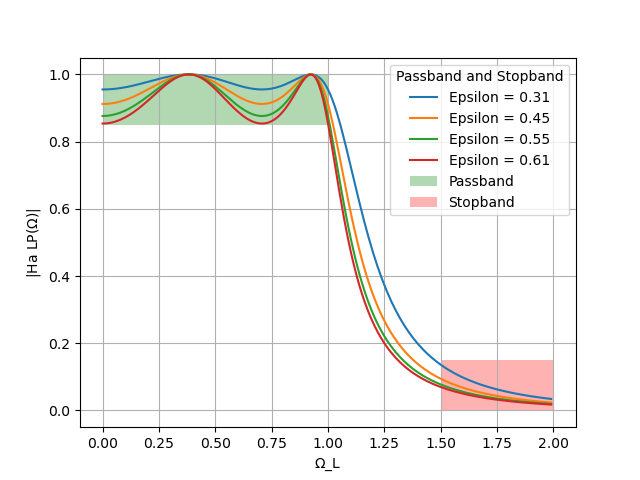
\includegraphics[width=1\columnwidth]{figs/1.png}
\caption{The Analog Low-Pass Frequency Response for $0.31 \leq \epsilon \leq 0.62$}
\label{fig:H_for_diff_eb}
\end{figure}

In \figref{fig:H_for_diff_eb} we can observe the equiripple behaviour in passband and monotonic behaviour in stopband. As the value of $\epsilon$ increases the value of $\vert H_{a,LP}(j\Omega_L)\vert$ decreases.\\

\item {\em The Low Pass Chebyschev Filter:} Thus, we obtain
\begin{equation}
\label{lpsqfinal}
\vert H_{a,LP}(j\Omega_L)\vert^2 = \frac{1}{1 + 0.16c_4^2(\Omega_L)}
\end{equation}
where
\begin{equation}
c_4(x) = 8x^4 + 8x^2 + 1.	
\end{equation}
The poles of the frequency response in (\ref{lpfirst}) lying in the left half plane are in general obtained as 
$r_1\cos\phi_k + jr_2\sin \phi_k$, where
\begin{eqnarray}
\label{lppoles}
\phi_k = \frac{\pi}{2} + \frac{(2k+1)\pi}{2N}, k = 0, 1, \dots, N-1 \nonumber \\
r_1 = \frac{\beta^2 - 1}{2\beta}, r_2 = \frac{\beta^2 + 1}{2\beta}, \beta = \left[ \frac{\sqrt{1 + \epsilon^2} + 1}{\epsilon}\right]^{\frac{1}{N}}
\end{eqnarray}
Thus, for N even, the low-pass stable Chebyschev filter, with a gain $G$ has the form
\begin{equation}
\label{poleleft}
H_{a,LP}(s_L) = \frac{G_{LP}}{\prod_{k = 1}^{\frac{N}{2}-1}(s_L^2 - 2r_1\cos\phi_ks_L + r_1^2\cos^2\phi_k + r_2^2 \sin^2\phi_k)}
\end{equation}
Substituting $N = 4$, $\epsilon = 0.5$ and $H_{a,LP}(j) = \frac{1}{\sqrt{1+\epsilon^2}}$, from (\ref{lppoles}) and (\ref{poleleft}), we obtain 
\begin{equation}
\label{lpfinal}
H_{a,LP}(s_L) = \frac{0.3125}{s_L^4 + 1.1068s_L^3 + 1.6125s_L^2+0.9140s_L + 0.3366}
\end{equation}
In Figure 2 we plot $|H(j\Omega)|$ using (\ref{lpsqfinal}) and (\ref{lpfinal}), thereby verifying that our low-pass Chebyschev filter design meets the specifications.
\end{enumerate}
\end{document}
